\documentclass{l4proj}

\usepackage{csquotes}
\usepackage{listings}
\usepackage[
backend=biber,
style=ieee
]{biblatex}

\usepackage{pgfplots}
\pgfplotsset{width=10cm,compat=1.9} 

\addbibresource{bibliography.bib}

\begin{document}
\title{Building Applications on the SAFE Network}
\author{David Brown}
\maketitle

\begin{abstract}

The SAFE Network is a decentralised peer-to-peer data storage network. To explore its effectiveness for use in software development, an application called SAFE Wiki was built. SAFE Wiki facilitates the storage and browsing of websites like Wikipedia on the SAFE Network. Through the evaluation, a number of potential issues with the adoption and use of the SAFE Network has been highlighted. The rigidity of how applications must be built presents challenges for software development. Whether these challenges can be solved dictates the ultimate success of the SAFE Network.

\end{abstract}

\educationalconsent

\tableofcontents

\chapter{Introduction}
\pagenumbering{arabic}

\begin{displayquote}
The SAFE Network is a decentralised data storage and communications network that provides a secure, efficient
and low-cost infrastructure for everyone \cite{safenetwork}.
\end{displayquote}

\section{The SAFE Network}

The SAFE Network \cite{safenetwork} is an open-source project being developed by a company in Scotland called Maidsafe \cite{maidsafe}. Their aim is to build "The World's First Autonomous Data Network". An `Autonomous Data Network' in simple terms is "...a network that manages all our data and communications without any human intervention and without intermediaries" \cite{autonomous-data-networks}. The network is comprised of \textit{vaults}. A \textit{vault} is a simple program that anyone can run on their computer. Together, all the vaults that comprise the SAFE Network work together to store and serve data. As anyone can run a \textit{vault}, the network (which again works autonomously) stores data in a decentralised manner. Owners of \textit{vaults} are compensated for their computers resources, which encourages more \textit{vaults} to join the network. Increasing its reliability, storage capacity and performance. A global network that facilitates the decentralised, highly redundant and secure storage of data creates exciting new opportunities for developers.

\section{Aims}

In this project I aim to not only explore the technical benefits the SAFE Network provides, but also consider the societal impact such a network could have. For the project I have developed an application that I have called SAFE Wiki. SAFE Wiki aims to provide \textit{permissionless} and decentralised access to Wikipedia, facilitated by storing an archive of it on the SAFE Network. ZIM\cite{zim} is a file format that provides a convenient way to store content that comes from the internet. A ZIM file is a self-contained entity that can hold `copies' of entire websites, such as Wikimedia content, for the purposes of viewing them offline. SAFE Wiki will be able to write the ZIM files to the SAFE Network and then provide the capability for anyone to browse them. 

Through building the application I hope to explore the architectural and developmental challenges in working with such a new project. With a working product it will then be possible to draw conclusions on whether or not having Wikipedia hosted on the SAFE Network will be useful to people.

\section{Motivation}

\subsection{Technical Impact}

Traditional software architectures that are commonly associated with the internet, such as client-server, cannot be used with the SAFE Network. Thus different architectural approaches must be taken when building the software that interacts with the network. It is always stimulating to work with new technology and the SAFE Network definitely promises that opportunity. Through this report I hope to not only convey my experience working with the SAFE Network, but also outline any flaws and issues I can see with both adoption and practical usage. This is in combination with exploring the new opportunities the network provides for softare development.

\subsection{Cultural Impact}

In my opinion, the right to liberty and the unobstructed access to information is the most important right we have. Throughout history, a common tactic of oppressive governments is to block access to information. By doing this they try to break down a culture. To control people. The most prominent example of this was the Nazi Book Burning Campaign \cite{book-burning}. The goal of this was to destroy any literature or information that could subvert the ideologies that Nazism is built upon.

\citeauthor{doi:10.1177/0165551506075327} propose that a true `Knowledge Society' cannot be achieved without freedom of information\cite{doi:10.1177/0165551506075327}. A `Knowledge Society' is defined by \citeauthor{binde2005towards} in \citetitle{binde2005towards}\cite{binde2005towards} to be a society in which the dissemination of information (knowledge) is open and collaborative. Specifically, the SAFE Network ensures the freedom of access to information. This is why I find the prospect of bringing Wikipedia to the SAFE Network to be such an exciting concept. The benefits to society when citizens are permitted the liberty to seek and consume new ideas cannot be overstated.

\begin{displayquote}
Article 19, Universal Declaration of Human Rights\cite{assembly1948universal}: \textit{Everyone has the right to freedom of opinion and expression; this right includes freedom to hold opinions without interference and to seek, receive and impart information and ideas through any media and regardless of frontiers.}
\end{displayquote}

\chapter{The SAFE Network}
\label{ch:thesafenetwork}

Decentralisation of data is the core benefit of the SAFE Network. As with many things in life, once someone has ownership or control of something they can either use that position of power for good purposes or for less desirable ones. The internet as it exists today is very fragile in this regard. When you upload a file to Dropbox\cite{dropbox} or OneDrive\cite{onedrive}, where does this file exist? Well that file exists solely on the servers that those organisations have control over. Once an organisation has data they can do with it what they please, acting within the bounds of overcomplicated privacy polices to manage your data. Not only does this incur the obvious privacy infringements (which we will not cover cover too much within this paper), but it can lead someone into the false sense of security that their data is safe. If for instance, someone managed to hack Dropbox or there was a catastrophic failure at the datacenter, who is to say that your data would be safe? That would depend upon a lot of factors such as: do they keep backups, do you yourself have a local copy of the file etc. On a much larger scale companies like Amazon provide AWS\cite{amazon-aws}, an enterprise grade cloud-computing platform. If AWS were to fail, or be targeted, many of the worlds biggest websites would cease to function. This is because this computational power, data is centralised. It is not necessarily an \textit{easy} target, but it is a single identifiable piece of the equation that if removed, causes the whole thing to collapse. This \textit{problem} is what the SAFE Network means to answer and is a question I will be exploring throughout this paper.

\subsection{Ownership of Data on the SAFE Network}

Accessing the SAFE Network is \textit{permission-less}. What this means is that you don't need to go to a central body that controls the network to ask for (register) an account. You simply connect to the network and create one yourself. This has big implications for how people can interact with the network. Once you establish a connection to the network and create an account, you have the same exact same rights and privileges as any other user on the network. You can retrieve any data that exists on the network (although you may not have the cryptographic keys to actually read that data) and store data if you have enough Safecoin. Safecoin is the \textit{cryptocurrency} of the SAFE Network, it is used to pay for the storage of data and to reward nodes for storing data\cite{lambert2015safecoin}. I will go into much further depth later on in the paper. Once a user has enough Safecoin, they can store any arbitrary data on the network that they wish. They can either make this data public, for instance sharing a photograph, or encrypt this data and do with the key what they wish. At a high level, an account is just a piece of data that is stored on the network. It is made up of an \textit{Account Secret} and a \textit{Account Password}. With both of these you can log into the network and interact with all the data you have uploaded to the network. Your \textit{Account Secret} and \textit{Account Password} never leave your client, they are not stored anywhere and are never sent in plaintext to the network (again I will explain this in much greater detail later). This means that \textbf{only} the person who has access to \textbf{both} the \textit{Account Secret} and the \textit{Account Password} can: see what data the account has written to the network, manage the privileges to the data and decrypt any data the account has used its encryption keys for.

In decentralised data storage networks, who owns the data is a difficult question to answer. The example we will examine is BitTorrent\cite{cohen2008bittorrent}. The SAFE Network shares some core characteristics with BitTorrent but deviates greatly on some others. The \textit{ownership} of data is one such point. In BitTorrent (and other decentralised data storage networks) who actually \textit{owns} the data. Is it the person who uploaded the torrent or is it collectively owned by everyone who holds a copy of that data? In the SAFE Network, the ownership of data is more clearly defined. When data is uploaded to the SAFE Network, the data is split up into chunks and distributed across nodes that makeup the network. The data is duplicated across different nodes (which introduces a level of redundancy) and is available for consumption by anyone who has the key to that data. If it was uploaded as \textit{public} data then anyone (with the correct address) can read that data. Fundamentally though, that data has an owner. The account that originally uploaded it to the network. They can do with it what they wish, including deleting the data permanently. This contrasts with BitTorrent greatly, wherein data cannot simply be \textit{deleted}. If you shared data on BitTorrent then wanted to delete it, you would have to communicate directly to each client that had a copy of the data and ask them to delete it. They do not have to comply with this request. Thus the SAFE Network having the concept of \textit{ownership of data} is very important as it opens up different use cases that haven't existed before.

Owing to this system of ownership, it brings about its own challenges in regards to the law. Data that has been written to the network is \textit{immutable} without the \textit{Account Secret} and \textit{Account Password}. It cannot be removed or deleted. This could mean that users could simply upload copyrighted/illicit material to the network as public, delete their \textit{Account Secret} and \textit{Account Password} and it will be available to everyone forever. Even if the original uploader was apprehended, they couldn't even delete the data if they wanted to as they have forgotten the necessary login to do so. This system is a natural consequence of the design of the SAFE Network. You cannot have a permission-less and decentralised data storage network that has a \textit{master-key} to alter data. To do so would undermine the security of the network as a whole, if such a key existed then bad parties would eventually discover it. A key concept is that users control their own data. Nobody else. If such a \textit{master-key} existed then this property of the SAFE Network would be \textit{broken} and its use cases diminished dramatically. Thus the uploading and distribution of illegal or copyrighted content could be a huge issue for the adoption of the SAFE Network. I have spent a great deal of time pondering this question, I see it as the biggest challenge the SAFE Network will have to overcome. People \textbf{will} use it to distribute copyrighted and illegal content, the SAFE Network is essentially the \textit{perfect} system to do so. This problem \textbf{will} become evident when the SAFE Network reaches full release. The biggest issue is user perception, take Tor\cite{tor} as an example. Many people in the general populous think of the 'Dark Web'\cite{dark-web} as a haven for all kinds of illicit activity. Thus when they hear of applications like Tor that can be used to access the 'Dark Web' they make this association. "Tor means illicit activity". This same problem \textbf{will} exist for the SAFE Network. I feel it is very important that Maidsafe realise this and take the proper precautions to educate people. At the end of the day, the SAFE Network is a tool. Like any other tool, people will most likely do bad things with it. The difficult question to answer is if the benefit it provides to \textit{good} people justify the benefits it provides to \textit{bad} people.
 
\section{Peer to Peer vs Client Server}

Centralisation of data and computing power is a natural consequence of the Client-Server architecture that has formed around the internet. Throughout this section, I will use \textit{Netflix}\cite{netflix} as an example to help illustrate my points. When you watch a video on Netflix, your device is merely a consumer of that data. A server owned by Netflix streams the video to your device and that is as far as the relationship goes. With this architecture, there are some obvious benefits. Mainly for the realm of rights management. As Netflix controls access to the data it holds (in this case video files) it is \textit{easy} for them to regulate access to it. They have complete control over what happens to that data. Let's contrast this with another, very popular, means of consuming video that works using a Peer-To-Peer architecture.

\subsection{BitTorrent}

The first stable version of the BitTorrent protocol was released in 2001. Since then it has become one of the worlds most popular means of file sharing and indeed internet traffic. Accounting for \%3.5 of global internet traffic at the time of writing\cite{bittorrent-usage}. In a \textit{permission-less} environment users are allowed to freely share files with one another. As there is no centralised body controlling who has access to what data, the system has been widely used for the \textit{piracy} of copyrighted material. The BitTorrent protocol helps to solve many of the same challenges that the SAFE Network aims to. One of which is the centralisation of data in a Client-Server architecture. In the BitTorrent protocol, peers form what is known as a 'swarm'. A 'swarm' is all clients that aim to download a a full copy of a piece of data. A piece of data is broken down into chunks and each chunk has a unique hash that allows clients to uniquely identify each piece of the original file. A client in the swarm is referred to as \textit{peer} when they don't have all the relevant pieces of a file. A client in the swarm is referred to as a \textit{seed} when they do hold all pieces of a given file. The 'resting state' of this network is when all clients in the swarm are \textit{seeds}. So clients will use peer-to-peer routing to send chunks of the file to other clients in the swarm that do not have it. This way of sharing data brings about many benefits. 

In BitTorrent there is no central 'server' to attack (disregarding a \textit{tracker}, there are \textit{tracker-less} solutions available). This means that you can lose clients from the swarm (or clients can leave and rejoin) and as long as at least one person in the swarm has a copy of a specific chunk of data all clients in the swarm can spread the data and become \textit{seeders}. This level of data redundancy is a huge benefit to BitTorrent over a traditional client-server model.

Data transfer costs are also a huge benefit to BitTorrent. In the traditional model, the owner of the server has incurs great cost in the hosting of the file. They have to pay for the management, storage and the network costs of sharing that data. For large companies this is often a negligible cost that doesn't impact on them, for smaller organisations however (especially non-profits) this server cost can be a big problem. This is a big reason why many Linux distributions so often provide BitTorrent links to download the operating system. By using BitTorrent they can offload the cost of sharing the file onto their users. This works almost on a good-samaritan basis. Where in if you download a file you really should aim to have your \textit{seed-ratio} hit at least 1 before leaving the swarm permanently (a clients \textit{seed-ratio} is how much of the file they serve to other users against how much they themselves have downloaded from the swarm). For the vast majority of users this cost is negligible and can act as a 'good-will' gesture to help support projects.

Data transfer speeds are a major positive of the BitTorrent protocol. When a client is acting as a \textit{peer}, their download speed is limited to the summation of the upload speeds of the clients they are receiving file chunks from. This means that in a well established swarm that your file will download as fast as your internet connection will allow. The more users that join the swarm, the faster and more resilient to failures the network gets.

This might all sound wonderful, but there is a glaring \textit{flaw} that means that companies like Netflix cannot use BitTorrent to offload network responsibilities to its users. That \textit{flaw} is control. Once shared, a video file cannot be easily removed from the network. This has big implications for things like Copyright, where they may only have the licence to provide access to a piece of content for a set period of time. I use the term \textit{flaw} very usefully, many people would indicate that this is one of BitTorrent's biggest benefits and I would agree with them. It is however important to realise that this is a limiting factor to organisations who could otherwise find use in the technology.

BitTorrent may solve many issues surrounding the distribution of files, but falls short of solving the decentralisation of the internet as a whole. The main limitation attributing to this is that data on BitTorrent is not mutable. Once a file has been spread to a swarm it is an immutable entity that cannot be changed. This limits BitTorrent to the sharing of files and not being able to do things like support dynamic websites, forums, email etc. (I want to emphasis that I don't mean this as a criticism of BitTorrent. It does one thing and does it very well. It has a proven track record of working and has laid the groundwork for other projects, such as the SAFE Network). The other attributing factor is that data only exists inside \textit{swarms}, you cannot interact with data without first joining the relevant swarm. So the discoverability of data is an issue. A given node within the network can't work out how to retrieve a chunk of data that is not located in the swarms it belongs to. These are all points that the SAFE Network aims to address.

\subsection{Serverless Architecture}

The idea behind a serverless architecture is to move as much computation/functionality to the client as possible. As time passes, the computational power that the masses have access to gets faster and faster. This computational power goes \textit{wasted} for the most part. When you browse the internet, interact with Facebook for instance, your computer actually does very little in terms of processing the information you are seeing. It does have to do work rendering websites and such but there is computational power going unused. Most, if not all, of the data is processed on FaceBooks' servers then merely served to you as a consumer. Your browser is a \textit{thin-client}. Not only does this incur vast operational costs for organisations, but it also means that information is being processed on their server that could be done locally.

In the SAFE Network, there are no 'servers' so to speak. The 'servers' on the network are what are called \textit{vaults}. I will give a deeper explanation of \textit{vaults} later in the report, for now just think of them as serving a similar purpose as to what nodes do in a BitTorrent swarm.  The only interaction a client has with the SAFE Network is the storage or retrieval of data, that it. So the SAFE Network in this capacity can serve a similar purpose to BitTorrent. Additionally what the SAFE Network has is the ability to route requests throughout the entire network. All \textit{vaults} in the network have knowledge of how to find a given chunk of data that exists on the network. This is different to BitTorrent because it can only find a chunk of data within the swarms it knows about. As this dynamic routing exists, the SAFE Network has a form of DNS that can be used. Another major difference is the SAFE Network is capable of mutable data. This means that the SAFE Network is fully capable of supporting dynamic websites, forums, email etc. You can open a browser that is capable of connectivity with the SAFE Network and browse the \textit{internet} just as you would normally. Only in this circumstance you are browsing an entire \textit{internet} supported by a Peer-To-Peer architecture.

At a high level, the only purpose a \textit{vault} serves is to store and serve data. That's it. This means that websites built for the SAFE Network must offload all the processing to the client and only use the network as its storage 'back-bone'. Thus the \textit{Serverless Architecture} model is a good fit for the SAFE Network. It allows you to build very powerful websites but keeps the processing of data local. This method of building websites has been around for a long time. With the advent of JavaScript and other such technologies, it was possible to dynamically change websites locally and run code locally without needing the server to do any processing. Very powerful JavaScript \textit{applications} can be served, think of online games. A website that serves these \textit{mini-games} doesn't do the processing for the game on their server. They merely serve the JavaScript/Flash/Java/Etc code to you and then your computer/client does all the hard work. Another of this are online \textit{office suites}, they are very powerful programs that can be ran through the browser. They depend heavily on the processing power of the user to provide them with an experience similar to what they could achieve with a desktop application. A true \textit{serverless architecture} model takes this to the extreme, there is absolutely no processing of data on the server. It is all done on the client. 

The way the SAFE Network operates forces the \textit{serverless architecture} architecture to be used (unless you merely use the SAFE Network as a component in your stack). This introduces challenges in that it is a new way of thinking about how to design websites and applications. Instead of complex servers, you almost entirely erase this concern from your development. You don't really need to consider how your apps data will be served, just how you go about accessing/storing it. Instead of designing websites the \textit{traditional} way, you develop them like you would a \textit{fat-client}. Websites will become heavier, requiring more care and optimisations. Messy and slow JS is abundant in the internet today, mostly due to the abundance of computing power that exists. Why spend time optimising when you can throw more CPU and RAM at it? This hap-hazard way of thinking cannot really exist for \textit{serverless architecture} websites or users will not have a great experience. An avenue that I think will become popular within the SAFE Network developer community is Web Assembly. 

Web Assembly is an assembly-like language that you can compile C, C++, Rust, etc, to and then run inside web browsers. It allows you to write code in high-level languages (that aren't interpreted like JS) and then serve it to users such that the code runs with \textit{near native} performance. This has big implications for the internet as a whole, not just the SAFE Network. A technology like Web Assembly could therefore be extremely useful when building websites that use the \textit{serverless architecture} model. It can give developers access to languages and frameworks to build websites that just weren't available before. As it promises near-native performance, it could be a great tool with which to build rich websites that aren't clunky and slow. Websites that run nearly as fast as desktop applications will therefore be possible.

\section{A Return to Fat Client Applications}

At a high-level, a \textit{Fat Client} is a computer (application) that can perform operations and tasks without relying on a central \textit{server}. A Fat Client may still need to make periodic connections to a server but the vast majority of its functionality can be performed without \textit{chatter} with the server. The concept of a Fat Client is juxtaposed to that of a Thin Client. Traditionally a Thin Client was a lightweight computer that relied heavily on a server to have any sort of utility. They would be able to perform some tasks locally but the vast majority would require a constant connection to a server. The traditional model of the internet, an overwhelmingly client-server based structure, has encouraged the growth of the Thin Client model. Historically this approach does make sense, computers were expensive and if you could centralise the required computational power you could reduce costs. In todays world however, computing power is fast and readily available. As discussed previously, this computational power (for the most part) goes to waste. Applications (specifically internet browsers) are acting as Thin Clients for content. Although not all Fat Clients follow the \textit{serverless architectural model}, applications that are designed to be \textit{serverless} are inherently Fat Clients. Hence because of the points mentioned previously, the SAFE Network encourages (almost requires) the Fat Client style of architecture.

This has vast implications for how applications should be designed for the SAFE Network and indeed influenced the choices I made for SAFE Wiki. Not only does one have to follow the design principles of the \textit{serverless architectural model}, but also that of the Fat Client. As Web Technologies grow, mature and develop it brings about new possibilities for how Fat Client applications can be used by end users. Instead of having to download applications to your device, new technologies allow rich \textit{serverless fat client} applications to be built and delivered through the web. A user simply needs to browse the internet as they already do instead of changing it to a model where they would have to download an app for Facebook, Twitter, YouTube etc. This style of \textit{content delivery} was not possible before, Web Technologies were not mature enough to support such rich experiences without relying heavily on server side processing. Hence I view the advent of new Web Technologies, such as Web Assembly that was mentioned above, to be an enabler in the success of the SAFE Network.

\subsection{An Example, Netflix on the SAFE Network}

Unlike BitTorrent, the SAFE Network could indeed be used to facilitate a service like Netflix. At its core, Netflix is about data. Their main goal being streaming the data that they have (video) to as many users around the world as possible and to do it as fast as possible. Although they would be able to benefit from redundancy and reduced server costs, there are flaws in the BitTorrent protocol that make it extremely difficult to justify it as a means of facilitating a website like Netflix. The biggest issue being ownership of data. As discussed previously, websites like Netflix have to have 'ownership of data'. They have to be able to control and \textit{mutate} the access of individuals to content. They simply cannot do this on BitTorrent. Another glaring whole in that approach is that of the health of the swarm. For content (data) to be available, nodes have to be online and sharing that file. This could mean that popular content would be readily \textit{seeded} but more obscure content may not be. The extreme of this being that the most obscure content might only be \textit{seeded} by Netflix themselves, resulting in a return to the Client-Server model they currently have. The SAFE Network solves these issues. Ownership of data is clearly defined, you own your data and nobody else does. Architecturally the SAFE Network insures that there are multiple copies of data spread around the network, meaning files will always be redundantly stored across the network. 

A Netflix style of service very much fits the \textit{Fat Client} style of architecture. Video playback is already processed locally so the content delivery system is the key part of the system that changes. Considerations to how things like 'Suggestions' would work are the biggest challenges in my opinion. Currently, that kind of feature fits the client server model quite well. Netflix gathers information about the shows you watch then suggests similar content that you might like to view. As this happens server side it is a continually updating entity that can improve and adapt, the inner-workings completely hidden from the user. With a \textit{serverless architectural} model this approach is simply unfeasible, There is no \textit{processing} of information on the SAFE Network. This would mean that to perform actions like 'content suggestion' you would have to perform it locally, client side. This applies to any application that is built on the SAFE Network. Users are quite used to visiting a service, such as Netflix or Facebook, and seeing newly \textit{generated} content that was created whilst their client was off. To account for this, new approaches in how to generate content will have to be thought of. This might be as simple as generating/processing the content when the user first opens the client and then displaying it to them. A more complicated approach might be to encourage users to keep applications open in the background so this processing can take place. In the browser this makes sense, users are familiar with the concept of keeping 'browser tabs' open. Often 'bookmarking' or 'favouriting' their favourite sites. One could envision a system wherein these 'tabs' would be refreshed in the background so users don't notice any delay when opening up the application (website). Traditional 'desktop' applications don't have this same luxury. Users typically 'quit' applications when not in use, so they would either need to be kept alive in the background (which may annoy some) or rely on quickly generating/processing content on startup.

\section{Alternative Business Models}

Like any new technology, the SAFE Network opens up many opportunities that didn't exist before. How the SAFE Network operates with \textit{Farming} and \textit{Safecoin} opens up new opportunities in how users could pay for content. In SAFE Network nomenclature, \textit{vaults} farm data. The safe and reliable storage (farming) of data is rewarded with \textit{Safecoin} which is a cryptocurrency built into the SAFE Network. One could envision an application that instead of charing users to use it, instead allows them to become a vault that generates Safecoin. This Safecoin could then be sent back to the creators of the program and hence financially compensates them for the usage of their application. A service like Netflix could very well make use of this kind of scheme, encouraging users to have their own vaults that then increases the performance of the network as a whole. One consideration of this approach however is that vaults don't get to choose what data they store, that is an integral part of the architecture of the SAFE Network. By following this financial model then it would be for the 'good of the whole', increasing the utility of the entire network and not just for one application.

This really is all about how to best use the processing power of the world. When a user sits and watches Netflix on an entertainment system, there is very little strain on the resources of the device. In the case of a games console, literally teraflops of processing power, advanced networking and storage facilities are going unused. Potential financial models can try to \textit{exploit} this untapped power to the benefit of both the user and the provider of the application. The most simple means I can see is to use that power to \textit{farm} \textit{Safecoin}. Not only increasing the utility of the SAFE Network but providing users with an entirely new way to pay for content. Offering the resources they have in exchange for access to services.

\section{Architecture of the SAFE Network}

The SAFE Network is still very much in active development. At the time of writing, the SAFE Network is currently on its second alpha revision (Alpha 2) out of a planned four. This not only made this project difficult because of a lack of documentation (I can't really blame them, it is not a 'finished' project), but means that anything I talk about in terms of the technicalities of the network is subject to change. In \textit{Chapter \ref{ch:architecture}} I will explain to the best of my ability how the network operates and functions \textbf{at the time of writing}. I don't expect much, if anything, to change in the near future. Just keep this in mind.

\chapter{The Architecture of the SAFE Network}
\label{ch:architecture}

The internet is constantly growing and changing. Changes in technologies slowly permeate throughout the network as if by osmosis. Governmental policy can have a large impact on how people interact with the network, whether that be Turkey blocking Wikipedia or the US abandoning Net Neutrality. This area is where the SAFE Network starts to deviate greatly from the \textit{traditional} internet. The SAFE Network is a 'Autonomous Data Network'. To have access to the SAFE Network means to have access to all of it. A government cannot curate access data. This is made possible by the architecture of the SAFE Network.

\section{Vaults and Clients}

The SAFE Network is comprised of \textit{vaults}. A \textit{Vault} is a singular program/application that a user runs on their computer, whether that be a server hosted in a datacenter, a Raspberry Pi or a desktop computer. A \textit{vault} is given a set amount of storage by the user which it then uses to \textit{farm} data. For a given \textit{vault} to join the network, it must pass a 'Proof of Resource'. This initial test is used to validate that the \textit{vault} has enough bandwidth and CPU power to be able to adequately perform its job. Similar to how a real world farmer looks after their crop/animals, a \textit{farmer} (\textit{vault}) on the SAFE Network looks after data. Understanding that nomenclature is quite useful in understanding the function a \textit{farmer} (\textit{vault}) serves. Once \textit{vault} is successfully storing data it is rewarded with \textit{Safecoin}, which is a cryptocurrency hosted on the SAFE Network. Reading data from the network doesn't incur any cost, it is only when writing data that a user (\textit{client}) has to expend \textit{Safecoin}. A user doesn't need to run their own \textit{vault} to interact with the network, all users interact through the use of a \textit{client}. To help increase privacy, a \textit{client} connects to the network through an intermediary \textit{vault} called a \textit{proxy node}. This \textit{proxy node} orchestrates the writing and retrieval of data on behalf of the \textit{client}, hiding the \textit{clients} IP address from the rest of the network.

The only time a user interacts with their \textit{vault} is through configuration before startup. The most notable configuration being the allocation of storage for the \textit{vault}. Once \textit{vaults} start communicating with each other there is no intervention by humans. The network itself votes on and decides many factors. This includes everything from where data should be stored to how much value a \textit{Safecoin} has. This is the autonomy of the network, it does not accept governance by humans and \textit{vaults} cooperate for the good of the entire network.

\section{Immutable and Mutable Data}

Similar to BitTorrent data is broken down into chunks. Each `chunk' of data that is stored on the SAFE Network is at most 1MiB in size and has a unique 256-Bit XOR Address. This allows every chunk of data to be uniquely identified and helps \textit{vaults} to decide who stores what data. Data stored on the SAFE Network can take one of two forms. It can either be \textit{Immutable Data} or \textit{Mutable Data}. A Mutable Data Structure (MD) is a \textit{key value} storage mechanism that allows for the storage of one thousand entries. An Immutable Data structure only stores a single ``value'', its address derived from the hash of the binary data it contains. An Immutable Data structure can itself only be 1MiB in size, but through the use of a \textit{Data Map} (Section \ref{subsec:self-encryption-data-map}) this limit can be subverted. As their names imply, Mutable Data can be freely mutated whereas Immutable Data cannot. It is this property of Immutable Data that eliminates duplication on the network. For example, if Bob uploads a picture to the network he is presented with the address of that file (possibly the address of a \textit{data-map}) and will have the relevant keys to access it. If Alice then uploads the exact same picture the data is not duplicated, she is simply presented with the same information that Bob was. If either Bob or Alice chooses to ``delete'' the picture, then their access to it is simply revoked as one of the them still has access to the picture.

\subsection{Self Encryption and Data Maps}
\label{subsec:self-encryption-data-map}

\begin{figure}[h]
	\begin{center}
		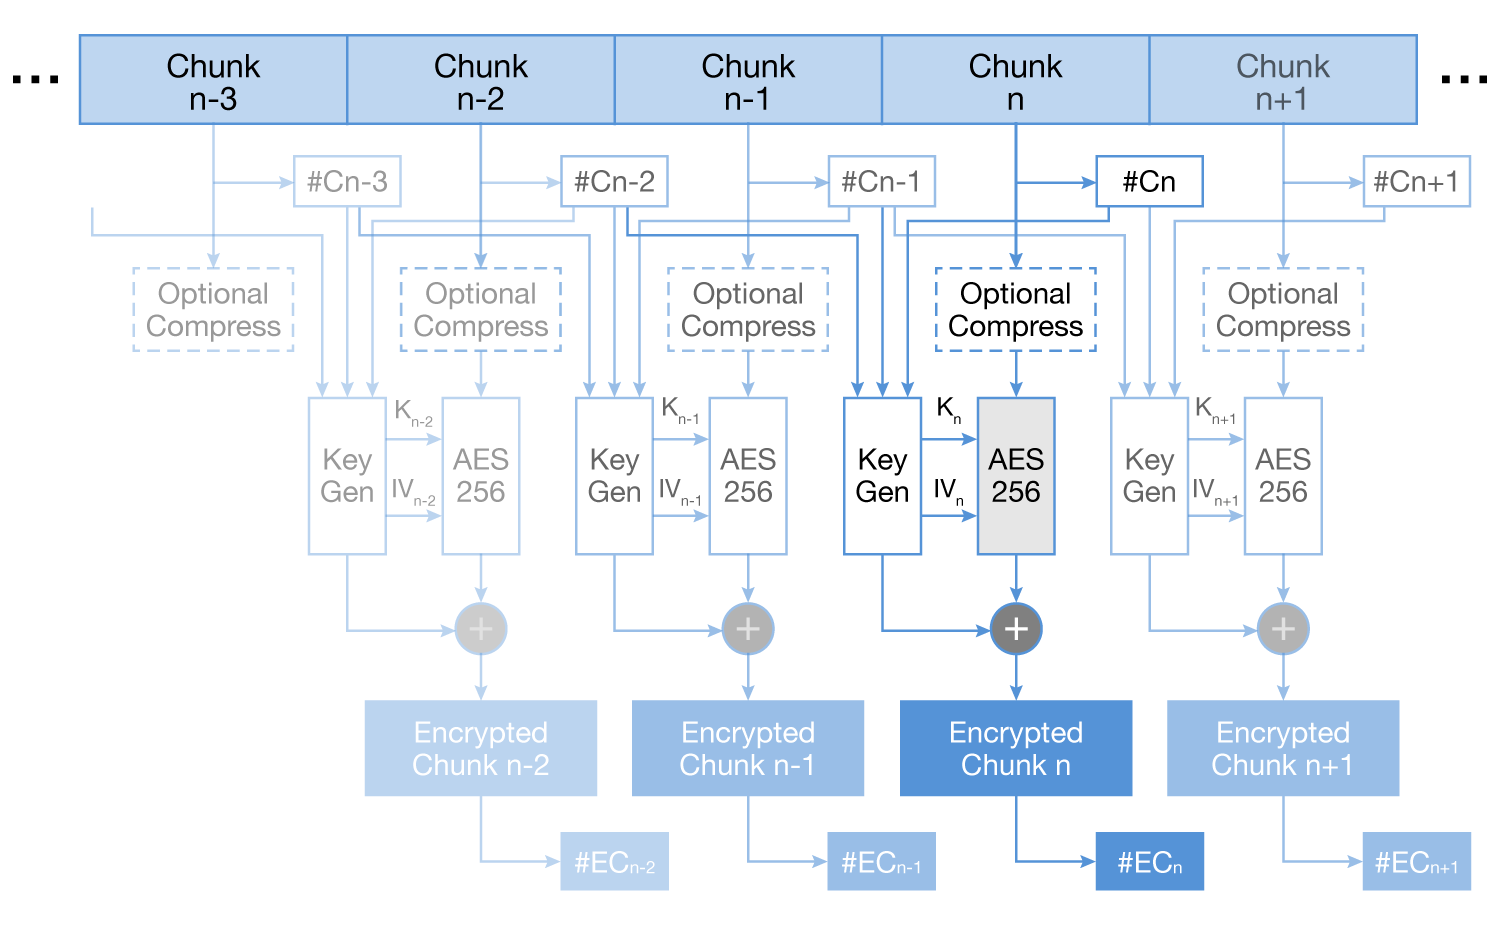
\includegraphics[width=\textwidth]{diagrams/self-encryption}
		\caption{The \textit{Self Encryption} process (sourced from https://safenetwork.wiki/en/Encrypt)}
		\label{fig:self-encryption}
	\end{center}
\end{figure}

Data that is stored on the SAFE Network goes through a process called \textit{Self Encryption}\cite{irvine2010self}. During \textit{self encryption} data is broken down into chunks of a specified size (The SAFE Network uses 1MiB chunks). To be able to reassemble and read the data a structure known as a \textit{Data Map} is created during the process. The \textit{Data Map} contains several pieces of information:

\begin{itemize}
	\item chunk\_num u32: Specifies how many chunks of data are within the Data Map
	\item hash Vec\textless u8\textgreater: Post-encryption hash of chunks
	\item pre\_hash Vec\textless u8\textgreater: Pre-encryption hash of chunks
	\item source\_size u64: The size of the original piece of data, before any encryption has taken place
\end{itemize}

The crucial structures of this \textit{Data Map} are the two vectors that store the pre-encryption and post-encryption hashes of chunks. The encrypted chunks of data are derived through the process of \textit{self-encryption}. What happens first is a piece of data is broken down into chunks and then hashed. The hash of the chunks is stored in the `pre\_hash Vec\textless u8\textgreater' of the \textit{Data Map}. This list is important as it defines the original piece of data before being encrypted. Each chunk then goes through an encryption process using AES 256. The key used for each chunk is the pre-encryption hash of one of the other chunks. The chunks then go through another step that further obfuscates the data. This step involves XOR'ing the data with the pre encryption hash of other chunks. A final hash is then taken of each chunk and stored in the `hash Vec\textless u8\textgreater' of the \textit{Data Map}. You can see the process of \textit{self encryption} in Figure \ref{fig:self-encryption}.

\textit{Self Encryption} is a generic process, there is nothing about it that specifically ties it to the SAFE Network. \textit{Self Encryption} is used to obfuscate data for storage, It is only with access to the \textit{Data Map} that you can make sense of the data. It is through this obfuscation process that means \textit{vaults} cannot distinguish what the chunks they are storing actually contain. It is just `garbage' data to them. This means chunks can be freely distributed across the network with the assurance that only the person with access to the \textit{Data Map} can read the original data.

\subsection{Disjoint Sections}

The unique address of every 1MiB chunk of data is used to determine what \textit{vaults} are responsible for storing it. Maidsafe's innovation was in the creation of what are called \textit{Disjoint Sections}. These \textit{sections} are groups of \textit{vaults} that are responsible for a certain range of the 256-Bit XOR Address Space. By default, the network requires a minimum number of \textit{vaults} to sustain the network. At the time of writing this is eight \textit{vaults}. These eight \textit{vaults} form a complete \textit{section} and are responsible for the storage of the entire 256-Bit address range. As more \textit{vaults} join the network, this \textit{section} will grow in size and then eventually split into two new \textit{sections}. There are numerous requirements that have to be met before a \textit{section split} is allowed.

% Insert equation for section split

\begin{figure}
	\begin{center}
		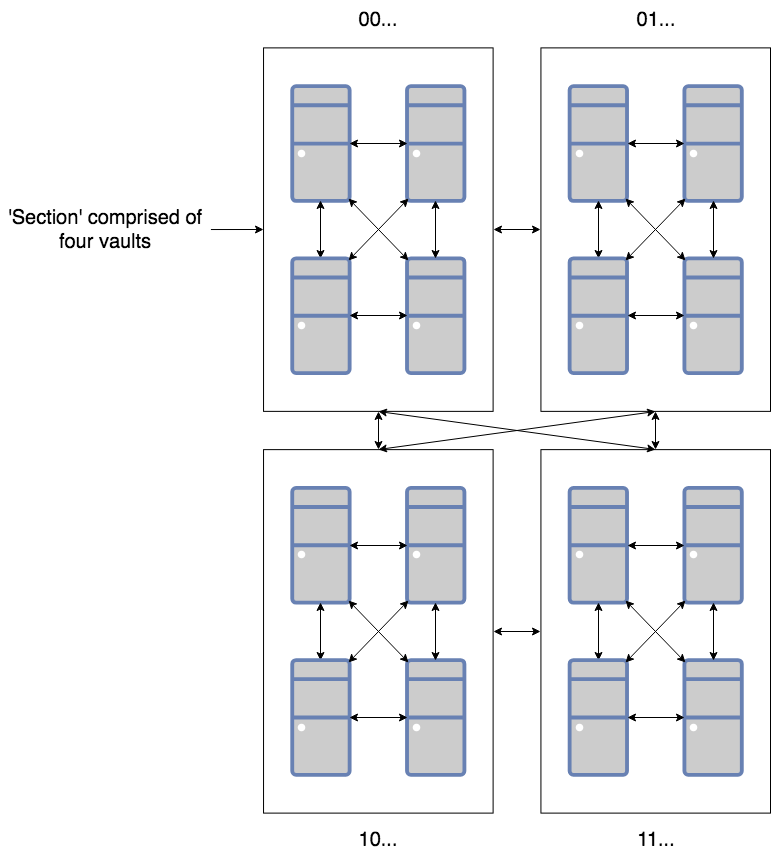
\includegraphics[scale=0.3]{diagrams/safe-network-sections}
		\caption{Four sections of a SAFE Network. You can see the address range each section is responsible for.}
		\label{fig:safe-sections}
	\end{center}
\end{figure}

After a split, \textit{sections} are then responsible for half of the 256-Bit address range that they were before. As more and more complete \textit{groups} of ~8 \textit{vaults} join the network, it continues to split and each \textit{section} is therefore responsible for the curation of less and less data. An important thing to note is that the SAFE Network doesn't assign 256-Bit addresses based on proximity, in a given section two \textit{vaults} could be very close together in 256-Bit XOR space but be located on different continents. This property helps the integrity of the network by ensuring \textit{vaults} in a given section are not located close to each other. Otherwise the network could be open to simple attacks. For example, start 8 \textit{vaults} on a single computer to form a \textit{section} then suddenly switch them all off which could cause data loss. If a significant number of \textit{vaults} leave the network then \textit{sections} have the ability to join with other \textit{sections} to ensure the stability of data is maintained. In Figure \ref{fig:safe-sections} you can see four \textit{sections} comprised of four \textit{vaults} each, you can see the address range that each \textit{section} is responsible for. In the diagram four \textit{vaults} make a \textit{section} instead of the traditional eight, this is just to make the diagram easier to process.

\subsection{Proof of Resource}
\label{subsec:proof-of-resource}

The \textit{proof of resource} (PoR) test is used to valid the effectiveness of a \textit{vaults} ability to store and serve data and is the value proposition of \textit{Safecoin}. The PoR is used to validate \textit{vaults} joining the network but also during other network events. Such an event is proving to its \textit{section} that it is indeed storing the data it says it is.

\subsection{Personas}

\textit{Vaults} can be characterised as having different ``Personas''. One such \textit{persona} is the \textit{Data Manager}. A \textit{Data Manager} is responsible for the storage of chunks within a a\\textit{section}. Their job is vital to the stability of the network. When data is stored on the network, it is actually replicated across multiple \textit{Data Managers}. At all times the network aims to keep a minimum number of copies of a chunk of data, if a chunk goes missing this chunk is replicated to another \textit{Data Manager} to ensure that data is stored redundantly. Hence within a given section, there will be several vaults storing identical chunks of data. Each having full knowledge of the chunks of data that the other \textit{Data Manager} hold. This scheme means that no \textit{vault} will ever hold the single copy of a chunk of data, meaning that data is stored redundantly across the network.

Another important \textit{persona} is that of the \textit{Client Manager}. A \textit{Client Manager} is responsible for storing the account data for clients that fall within its address space. When you create an account on the SAFE Network the data is stored on the network just like any other piece of data. It has a given 256-Bit Address and contains information like: how much \textit{Safecoin} an account has, the number of chunks of data that has been uploaded, etc. As an account is a 256-Bit address it will fall within the domain of a particular section, the \textit{Client Managers} in that \textit{section} will then store the relevant data.

\subsection{Accounts}

Accounts on the SAFE Network are special in that they are stored along with other pieces of data on the network. There is no centralised body or organisation that is needed to grant access to the network. An account on the SAFE Network is derived from two parts, an \textit{Account Secret} and a \textit{Account Password}. From these two components a client can gain access to a piece of data that is know as a \textit{Data Atlas}. A \textit{Data Atlas} contains a great deal of information:

\begin{itemize}
	\item The Safecoin balance of the account
	\item Address(es) of \textit{Data Maps} that the account has decryption keys for
	\item Decryption keys for the aforementioned \textit{Data Maps}
	\item ...
\end{itemize}
	
It is with this \textit{Data Atlas} that a user can interact with the network. A single login secures all of their data behind multiple layers of encryption meaning they just need one set of credentials to access the network and their data. An important caveat in this is that once credentials are lost, the \textit{Data Atlas} can never be read again. This is not a real problem for ``professional'' users as most make use of password managers and other such tools. At some point though even the most ``pro'' user could lose track of a password and with that their data is gone. There is no chance of recovery. This could involve losing irreplaceable data which can be heart-breaking for individuals and bankruptcy causing for companies. Thus keeping credentials safe is extremely important. This could be a prohibiting factor to a lot of users however, some may just not want to take the risk.

\section{Crust and Encryption}

\textit{Crust} is the secure routing layer designed and built by Maidsafe to provide the secure communications backbone of the SAFE Network. \textit{Crust} allows for reliable P2P connections and provides encryption for all traffic. Several Transmission Protocols can be used, falling back to UDP from TCP (for example) if required. Encryption at this level means that Data on the network is always encrypted, data is only decrypted client side and whenever it is not on a clients computer it is fully encrypted.

Encryption is a very important aspect of the SAFE Network. Whenever data is stored on the network, it is encrypted. Data on the network exists as discrete 1Mb chunks, each with its own 256-Bit Address. When a file is uploaded to the network, it undergoes a process known as \textit{self encryption}. As mentioned in Section \ref{subsec:self-encryption}, \textit{Self Encryption} is a technique that is used to break data down into 1MiB chunks and also to encrypt each chunk. These are the chunks that are ultimatly stored by \textit{vaults}. You can choose to have data ``unencrypted'' or what Maidsafe calls ``Plain'', what this means is that any user that knows the address of the data (and the type-tag) can retrieve and read the data. The special thing about this is that the data is still fully encrypted on the network through \textit{self encryption}, a \textit{vault} owner cannot decipher what the chunk of data holds. When anyone goes to access this data though, it is reassembled and you can read it. The two other types of encryption supported are Symmetric and Asymmetric. Through different key exchange mechanisms you can use these forms of encryption to build interesting applications.

\begin{figure}
	\begin{center}
		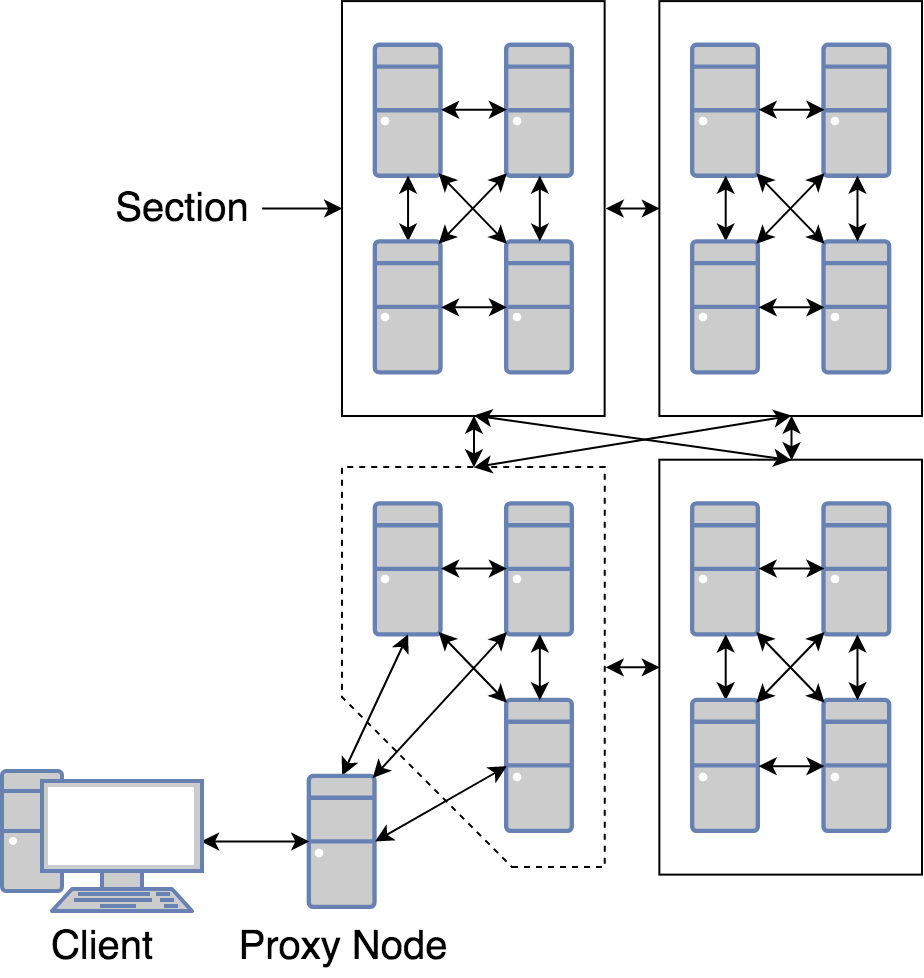
\includegraphics[scale=0.3]{diagrams/safe-network-connection}
		\caption{A client connecting to the SAFE Network through a Proxy Node}
		\label{fig:proxy-connection}
	\end{center}
\end{figure}

When a client connects to the network they do so through the use of a \textit{Proxy Node}. A \textit{Proxy Node} is a \textit{vault} that is used to liaise between a client and the network at large. The \textit{Proxy Node} is used to hide the clients IP address from the rest of the network. Beyond the proxy and deeper into the network all \textit{vaults} know is the XOR Address of the account being used and its Public Key. Hence by using a \textit{Proxy Node}, the real world identity of the client is well hidden from the rest of the network. This means that a given \textit{vault} cannot detect that the data it is sending is going to a certain geographical location. In Figure \ref{fig:proxy-connection} you can see the topology of how a client connects to the SAFE Network.

\section{Safecoin and Farming}

Safecoin\cite{lambert2015safecoin} is the cryptocurrency of the SAFE Network, it is earned by \textit{farmers} and spent by writing data to the network. The expectation is that as the cost of CPU/Storage falls with time, the value of the Safecoin will increase. Value in this context is how much data each coin facilitates the storage of.

When a user creates an account on the network, they are given a \textit{Safecoin} wallet. This wallet can be used to securely store the \textit{Safecoin} that belongs to the account. Akin to \textit{Bitcoin}, \textit{Safecoin} is a cryptocurrency. It can be sent between users in a permission-less manner. \textit{Safecoin} can be sourced in a number of ways including through \textit{farming} and by simply purchasing them with another currency. The ultimate purpose of \textit{Safecoin} is to incentivise people to run \textit{vaults}. Running a \textit{vault} is costly, so the reward of \textit{Safecoin} is used to incentive the participation of nodes in the network.

\textit{Farming} is the action of \textit{vaults} to store, maintain and serve data to clients. When a client requests a chunk of data, the \textit{vault} that successfully returns that piece of data will be given the opportunity to earn \textit{Safecoin}. The probability of being awarded this attempt to earn \textit{Safecoin} is determined by the \textit{farming rate} of the network at that specific moment in time. The \textit{farming rate} is used to balance supply and demand of data on the network. The SAFE Network tries at all times to keep a minimum amount of network capacity free, this is around \%30. When free space starts to fall below this threshold then the \textit{farming rate} will increase, meaning \textit{vaults} have the opportunity to earn more \textit{safecoin}. This works in the opposite direction too. If the network capacity grows so that there is an overabundance of free space then the \textit{farming rate} will decrease meaning \textit{vaults} earn less money. This constantly varying \textit{farming rate} is hence used to balance network resources and de-incentivise users adding \textit{vaults} with very high capacity to the network (if it is not needed). It encourages more \textit{farmers} when the network is running low on capacity (compared to demand) and discourages them when resources are overabundant.

The economics of \textit{Safecoin} are a subject that is out-with the scope of this paper. In short, its utility on the SAFE Network is not tied to whatever its `exchange price' is. Overtime, the storage `buying power' of each \textit{Safecoin} should increase as computing power and storage becomes cheaper. \textit{Safecoin} is in its infancy and indeed has not yet been implemented. This means it is subject to changes (however this is unlikely) from what has been described above. There are proposals upon how to build the \textit{Safecoin} support structure into the SAFE Network but as it has not been implemented yet I will avoid going discussing it in this paper.

\section{Quorum and the Datachain}

As the network acts as an autonomous entity there has to be some method for a given \textit{vault} to reach consensus with other \textit{vaults}. This problem is what Cryptocurrencies aim to solve through processes such as mining. \textit{Mining} is essentially the network reaching consensus upon what has happened (in this case, financial transactions). In the case of \textit{Bitcoin}, every time a block is \textit{mined} it is cryptographically linked to the block that came before it. As this \textit{Blockchain} grows in size, the consensus on past transactions grows and grows. For \textit{Bitcoin} and similar \textit{cryptocurrencies}, to be able to undo a transaction/block you would need to have control of over \%50 of the networks \textit{mining} power. The SAFE Network needs a similar mechanism on how to reach consensus. Analogous to a \textit{Blockchain}, the SAFE Network has a \textit{Datachain}. 

The Datachain is used to help insure the integrity of the network and can be used to help rebuild it in the case of a catastrophic failure. For any action on the network to be valid, whether this be the storing/mutation of data or a \textit{vault} joining a \textit{section}, there has to be a corresponding \textit{group signature}. This \textit{group signature} is stored in the \textit{Datachain} that all \textit{vaults} in a \textit{section} have. In order for an action to be considered valid, a \textit{section} has to reach a quorum. For a network where the minimum \textit{section} size is eight, a quorum would be five out of the eight vaults voting in agreement. This means that in a given \textit{section}, several \textit{vaults} could be acting as ``bad parties'' but network integrity wouldn't be lost. XOR Distance also comes into play in this process. The closer two \textit{sections} are in 256-Bit XOR Address Space the more they know about the data the other \textit{section} is storing. They will have access to the portion of the \textit{Datachain} that is used by that \textit{section} that is used to record data writes and mutation. This way a given \textit{section} can help to verify that a neighbour is acting as a good party in the network and that data being stored there has not been tampered with. The further away in 256-Bit Address Space two \textit{sections} are then the less they know about each other. This means that as the number of \textit{sections} increases, the influence a given a \textit{section} has over the network decreases. Eventually resulting in no \textit{section} in the network having an overview of the entire network.

A protection mechanism exists in the retrieving of data for when a vault tampers with data after it has been recored in the \textit{Datachain}. When a client requests a given piece of data, a single \textit{vault} is chosen to return that chunk of data. Alongside the data that is returned, a minimum number of acknowledgements from other \textit{vaults} in the section must be returned too. This way, a client can then verify the data they receive against the acknowledgements from the other vaults in order to ensure that the data is valid.

The development of the \textit{Datachain} is still very active, at the time of writing I have tried my best to summarise the current proposals. Thus the \textit{Datachain} is still very much subject to rapid range.

\subsection{Node Age and Churn}

A crucial part of the integrity of the \textit{Datachain} is \textit{node ageing}. For a \textit{vault} to \textit{vote} on network activity (this is the signatures that form the \textit{group signature}) it has to have proved itself a reliable node. A \textit{vault} cannot just join the network and start voting in network decisions. When a new \textit{vault} announces itself to the network, it is issued with the \textit{Proof of Resource} that was discussed in Section \ref{subsec:proof-of-resource}. If it passes then as long as the assigned \textit{section} reaches a quorum the \textit{vault} will join that \textit{section}, recording its membership in the \textit{Datachain}. This node is very ``young'' in the eyes of the network and as such is not trusted. It is not allowed to vote in group actions and is responsible only for the storage and transmit of data. A very interesting aspect of the SAFE Network is the concept of \textit{churn}. 

\textit{Churn} is used to constantly 'rotate' vaults round different \textit{sections} on the network. This means that in a given time frame, a \textit{vault} will not be responsible for the same 256-Bit address range. This important feature helps to ensure that it is very difficult to track down where data is stored in order to erase it or corrupt it. During churn, young \textit{vaults} with a lower \textit{node age} will be chosen more frequently than older \textit{vaults}. The \textit{vaults} chosen are assigned to new \textit{sections} to which it must give another \textit{proof of resource} to be allowed to join. If the new \textit{section} reaches quorum then the \textit{vault} joins and its \textit{node age} is incremented. Thus, trust must be earned by acting as a good party in the network over time. Only when a \textit{vault} reaches a certain \textit{node age} does it become an \textit{elder}. An \textit{elder} is a node which has the highest possible \textit{node age}, meaning it has has proven itself to be a reliable party over the course of time. When a \textit{vault} is an \textit{elder}, it gains the voting rights that eventually lead to the construction and maintenance of the \textit{Datachain}. If a\textit{vault} acts out of order then its \textit{node age} can be decremented or eliminated entirely. Trust must be earned.

\textit{Node ageing} and \textit{churn} are hence essential security features of the network and make it very difficult for an attacker to have any choice in the \textit{section} of the network they wish to attack.

\chapter{Implementation of SAFE Wiki}

SAFE Wiki is an application that allows users to both upload and browse content that can be stored in a ZIM file. The ZIM file format allows you to easily store content from the web, one of its uses is in the distribution of Wikimedia based content.

\section{Kiwix}

Kiwix first launched in 2007 as a way to browse the internet ``offline''. It achieves this through the use of ZIM files which are suitable for storing most HTML based content. One of the primary goals of Kiwix is to allow users to browse Wikipedia and other projects from the Wikimedia foundation without an internet connection. Whether this be in the middle of the ocean, Africa or even inside North Korea. Since the initial launch, different versions of the software have been released. Versions support many different platforms including: iOS, Android, Windows Phone, FireFoxOS, macOS, Windows and Linux. A user opens the app and then through a file explorer (or other means) selects the target ZIM file. Kiwix then presents the user with an almost ``web browser like'' experience. With resources like Wikipedia it looks uncannily like the real thing. Users have the ability to follow hyperlinks around the website (ZIM file) and search for pages. The London page of Wikivoyage can be seen in \textit{Figure \ref{fig:kiwix-firefox}}. With such a fantastic history behind the project, Kiwix was seen as the natural foundation to build SAFE Wiki upon. Kiwix is inherently a \textit{Fat Client} style of application as all processing is done on the client. Hence building upon an already \textit{Fat Client} application made perfect sense considering the points made in Chapter \ref{ch:thesafenetwork}. SAFE Wiki would do all the processing/reading of the file locally and use the SAFE Network as the storage medium for ZIM files.

\subsection{Kiwix JS}

Kiwix JS is a JavaScript variant of Kiwix, originally part of the Evopedia project it presents Kiwix in the form of a browser extension. This extension has support for many different environments (FireFox, Chrome, Edge, etc) due to the portable nature of Javascript.

As the SAFE Network is still very much in its infancy the developer API's reflect this. At the time of writing the only API's that are ready for use are the \textit{Node.js API} and what they call the \textit{Web API}. The \textit{Web API} can be used to build websites to interact with the SAFE Network whereas the \textit{Node.js API} facilitates the development of desktop applications. Both of these require the usage of JavaScript, hence forking Kiwix JS to build SAFE Wiki made logical sense.

\begin{figure}
	\begin{center}
			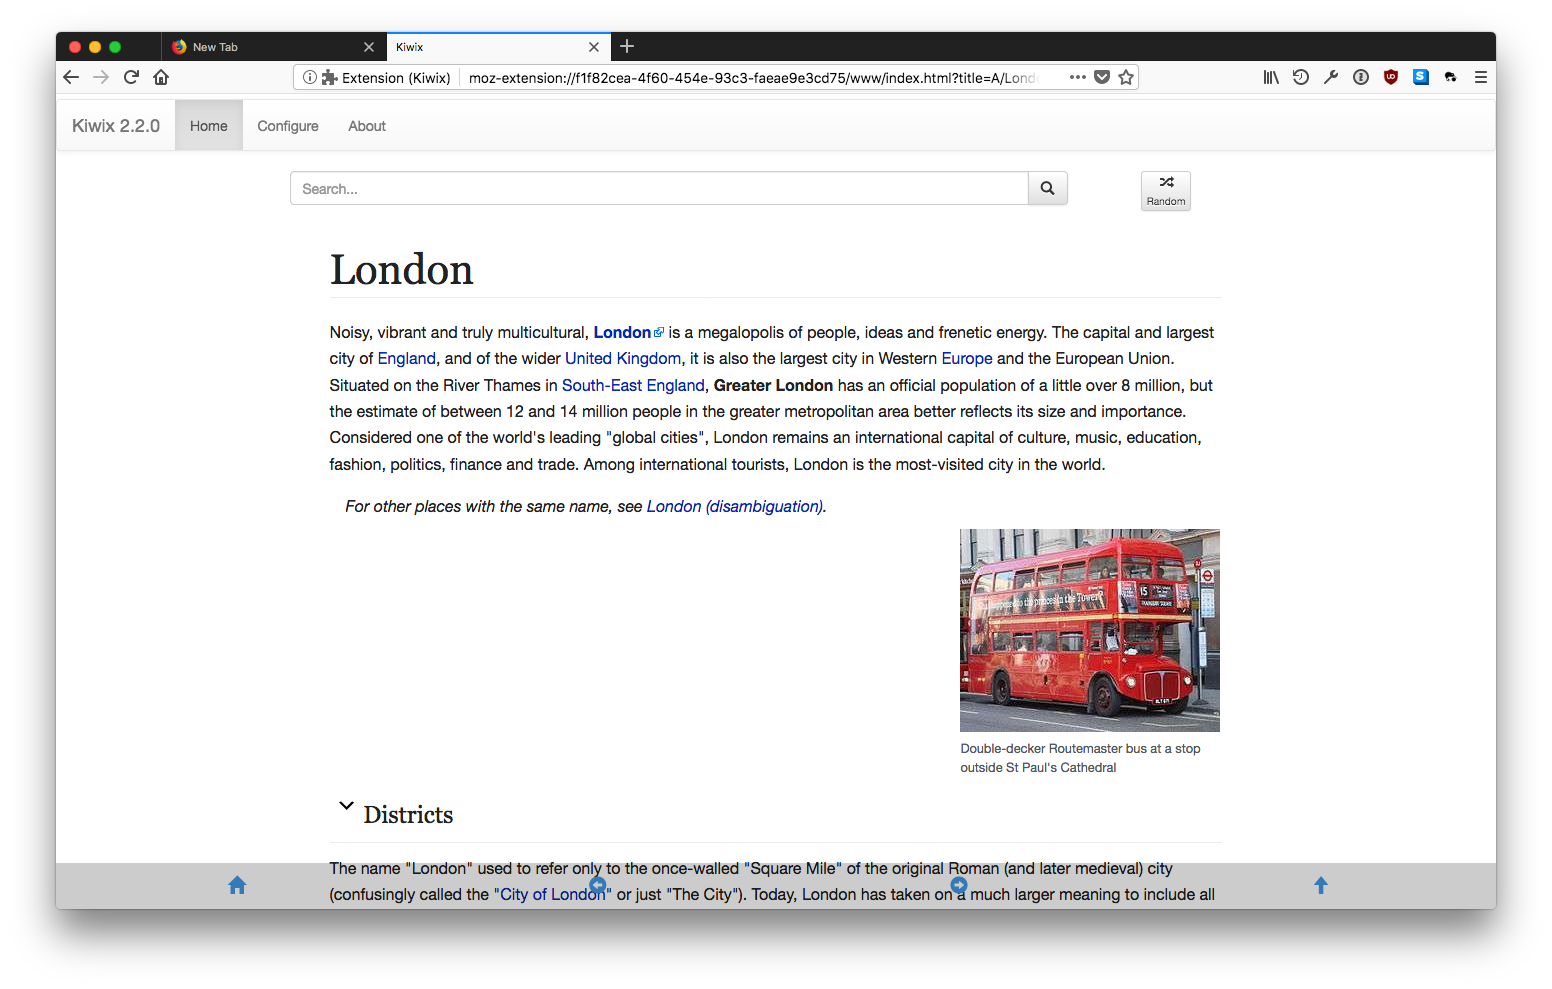
\includegraphics[width=\textwidth]{images/kiwix-js-extension}
		\caption{Kiwix-JS running in FireFox}
		\label{fig:kiwix-firefox}
	\end{center}
\end{figure}

Kiwix JS as it stands has support for Wikimedia and StackOverflow ZIM files (although others may work, just not supported). This meant that that through SAFE Wiki it would be possible to not only browse Wikimedia content but also content coming from StackOverflow. The content that users would be able to browse would be static, ZIM files are not mutable. The ZIM files being static does however bring its own benefits.

\section{Static versus Dynamic Content}

When the idea to ``build a Wikipedia on the SAFE Network'' was born, we were very well aware of the fact that it might just forever be a ``tech demo''. Getting enough users to start contributing content, and building an environment where strict moderation could occur, would have been a fools-errand given the time permissible for this project. It just wouldn't have been able to build a full Wiki system on the network and do it justice.

It is with that realisation that lead to the discovery of Kiwix. Instead of trying to build a Wiki system on the SAFE Network and trying to bring users across, it would be possible to bring Wikipedia (and other sites) to the SAFE Network. The content would not be dynamic in anyway (meaning the content couldn't be mutated) but it would be there for consumption. An important thing about this approach is that by the end of the year there would be a way to store a browsable copy of Wikipedia on the SAFE Network. In its entirety. Not just a simple throwaway tech demo but a tool that people might actually be able to use.

Websites like Wikipedia only work because of their user base. When a user edits an article this change is logged and anyone can review the changes made. As there are thousands of users anything that is grievously wrong is likely to be flagged and addressed quickly. If someone is acting as a \textit{bad-party} and editing pages wrongfully they can be blocked based on IP address. A simple example is a school, It does not need explaining that school children can be known for being rather silly sometimes. This behaviour can result in the vandalism of some Wikipedia pages. In such cases Wikipedia has the moderation tools to block the IP address(s) that belongs to a school (from making edits) and prevent any further vandalism. On the SAFE Network, this approach is impossible. A user could simply create another account and vandalise an open wiki all they want. It is for reasons such as this that building a dynamic wiki (with adequate moderation techniques/tools) would have been very difficult. A static mirror of Wikipedia was however very achievable.

A static version of Wikipedia might at first seam quite rigid, but in the context of the SAFE Network it makes sense. As the network has a concept of \textit{ownership of data}, a ZIM file can be directly tied to the original uploader. The ZIM file ``belongs'' to the account who uploaded the file and created the \textit{Data Map}. An organisation like Wikimedia, or a trusted third-party, can then upload ZIM files to the network with the assurance that users will know it came from them. It will then exist on the network as an un-censorable mirror (or archive) of whatever source the ZIM file came from. Everyone that has access to the SAFE Network can browse it, the only person that is allowed to ``remove'' access to the \textit{Data Map} is the original uploader. As long as a user trusts the source of the ZIM file and the address given to them for that file, they can \textit{trust} that the information contained within it came from them.

\section{Electron}

Electron allows you to ``Build cross platform desktop apps with JavaScript, HTML, and CSS''. Being able to produce an application that was cross platform was very important. The SAFE Network is not platform specific so SAFE Wiki should not have been either. As Kiwix JS is built upon web-technologies, Electron seamed like the obvious answer as to how to pull Kiwix JS outside of the web browser. Electron combines \textit{Node.js} and \textit{Chromium} into a single environment that can be deployed to the three main platforms: Windows, Linux and macOS. As there exists a \textit{Node.js API} for the SAFE Network it meant that a single application could be built. An application that could handle both the publishing of ZIM files and facilitate the browsing of them. The decision not to use the \textit{Web API} was because of file uploading. To facilitate the upload of large files, (The ZIM for Wikipedia with images is \textgreater 70GB) it really needed to build a desktop application.

\begin{figure}[h]
	\begin{center}
		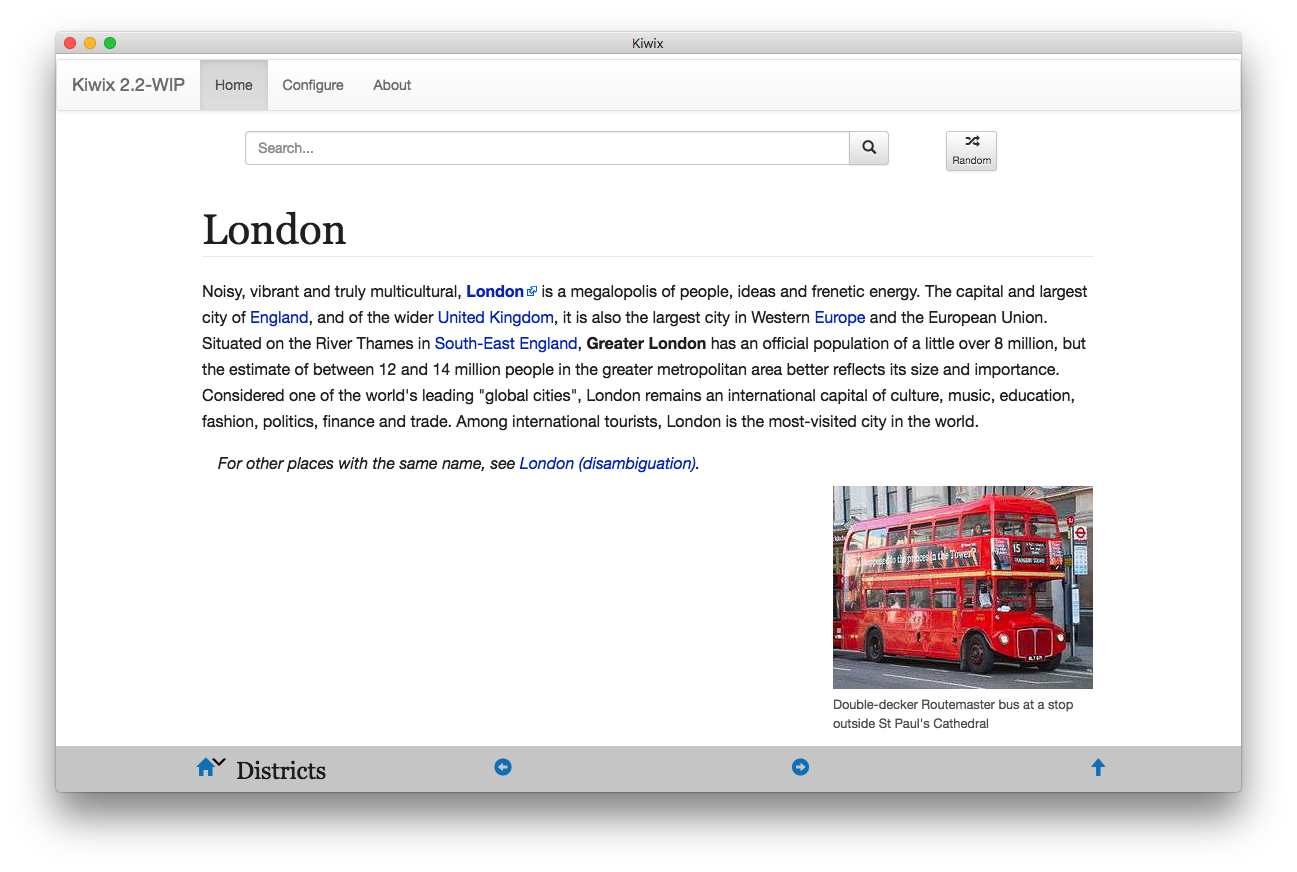
\includegraphics[width=\textwidth]{images/kiwix-js-electron}
		\caption{Kiwix JS as an Electron App}
		\label{fig:kiwix-js-electron}
	\end{center}
\end{figure}

Electron and \textit{Node.js} were unfamiliar technologies when development started. Making Kiwix JS run as an Electron application was hence quite a challenge. After a few months of work Kiwix JS was running in a desktop application. Indeed the creators of Kiwix had a similar idea of bundling Kiwix JS into an Electron application some time ago. They were pleased when contacted about the early success of this project. What was now SAFE Wiki (which can be seen in Figure \ref{fig:kiwix-js-electron}) could browse ZIM files from local storage and maintained all the functionality of Kiwix JS.

\section{Developing with the SAFE Network}

The SAFE Network was exceedingly difficult to work with, this was down to the lack of documentation and developer resources. Being only at `Alpha 2' they still have a long way to go before a true `1.0' release of the product. It is down to this development roadmap that indicates they are holding off on writing proper documentation until closer to the full release. The only saving grace in this matter was the Developer Forum. The Developer Forum is a very lively place with constant chatter, everyone pitches in and shares ideas. All the information needed to build SAFE Wiki was contained within the forums. This was not an optimal way to find the knowledge needed, it made work very slow and much harder than it needed to be. The lack of documentation and \textit{cannon} knowledge on certain topics resulted in the creation of several forum posts to help support this project. Users could not have been more helpful and most queries posted were resolved within a matter of days.

Development first starts with how to orchestrate the connection to the network. During development SAFE Browser was used, a fork of the Beaker Browser project. SAFE Browser takes the form of a web browser. Through it you can authenticate yourself with the network and browse any websites that are hosted on the SAFE Network, just like you can with a ``traditional'' web browser. If you build a standalone application, like SAFE Wiki, you can use IPC to communicate with SAFE Browser to gain authentication with the network. Once you have authentication you can communicate with the network directly meaning you don't need to use SAFE Browser as a middle man. Currently Maidsafe are working on the successor to SAFE Browser called Peruse. 

\begin{figure}[h]
	\begin{center}
		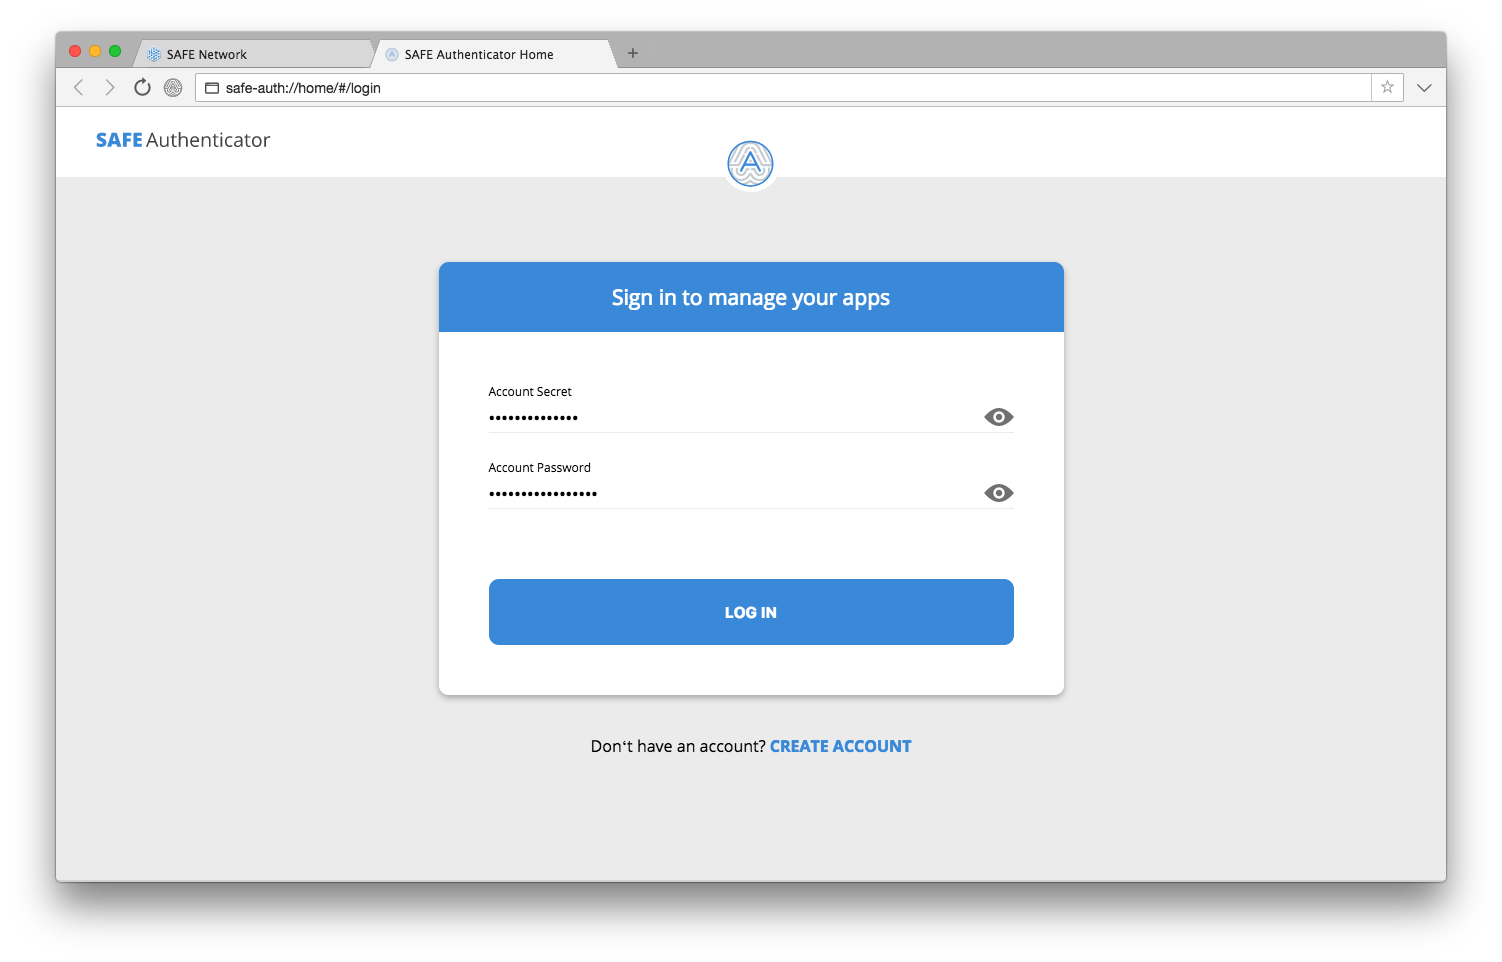
\includegraphics[width=\textwidth]{images/safe-browser-login}
		\caption{Login screen of the SAFE Browser}
		\label{fig:safe-browser-login}
	\end{center}
\end{figure}

To develop with the network you need to have some way of running your own ``development'' SAFE Network. There are currently three ways of achieving this.
\begin{itemize}
	\item Alpha 2 Network: This public network is hosted and ran by Maidsafe themselves. It is the ``official'' network for early adopters to host websites and run applications against. As it is a public network, it is not optimal for developmental work.
	\item Mock Routing: Mock routing is a technique that is baked into the SAFE Browser and Peruse. What it does is spoof the underlying network to the client through the use of a local database. This means that the client thinks it is talking to a real network while in actuality it is talking to a database. This is a very reliable way of developing locally, although it doesn't give you the full experience of how your application/web-site would work with a ``real'' SAFE Network. What this method does offer is simplicity. As it is built into the SAFE Browser you only need to download that single application. You just start SAFE Browser (with mock-routing support turned on) and you just work with it as you please.
	\item Local Network: Running a local SAFE Network is my preferred choice. Sadly it was very long into development before it was discovered just how easy it was to run a ``real'' SAFE Network locally. The process isn't as simple as downloading the binaries and clicking run, but it is not difficult. One has to download and compile the ``safe\_vault'' from Maidsafe's GitHub. This is a \textit{vault} that makes up the nodes of the SAFE Network. Once you have it configured, you then start up several vaults and they will automatically connect to one another. Once you have reached the ``min\_section\_size'' you set, then you can reliably start using the network for development. The ``min\_section\_size'' setting is used to configure the minimum number of vaults required to form one complete \textit{section} on the network and the default number is eight. It is possible to set this number lower (e.g. two), which makes running the \textit{vaults} on one machine much easier.
\end{itemize}

\subsection{Web Hosting Manager Example Application}

Maidsafe themselves provide a number of Electron example applications\cite{example-apps}. Looking through the code and how they worked was very helpful in figuring out how the \textit{Node.js API} actually worked. A big challenge for this project was just trying to figure out how SAFE applications should be designed, how they should authenticate themselves with the network and such. Design patterns for how to do a lot of these things will be established and grow naturally as more developers start working with the SAFE Network. For the purposes of this project, the style of how the ``Web Hosting Manager''\cite{web-hosting-manager} example app worked was very appealing. Web Hosting Manager is an application that can be used to upload websites to the SAFE Network. As such, it uses almost all of the API for numerous purposes which was brilliant for learning. Looking through the code it became apparent that there was a lot of repeating code across the example applications. It might be best described as ``boilerplate'' code. This led to the decision to simply ``fork'' the internal workings of Web Hosting Manager into SAFE Wiki instead of repeating the same code as Maidsafe themselves had done. SAFE Wiki's interaction with the SAFE Network is simpler so only the core functionality was taken. Most notably was the code for reading local files to then upload to the network. As mentioned previously there really are no guidelines on how applications should be built, so by forking this code it meant that development could follow the style that Maidsafe themselves had intended. Proper attribution has been added to any and all source files that are not of my own creation, this includes files from Kiwix JS. Most files have seen significant changes to them as I developed my solution and my own style of doing things, the complete history of the changes can be seen on the SAFE Wiki GitHub page.

\section{Authentication}

For an application to have connectivity with the SAFE Network it has to be authenticated. Regardless of whether it is a website or a standalone application. Communication from SAFE Wiki to the SAFE Browser for authentication was one of the most difficult parts of this project. As Electron allows (encourages) cross-platform development, what worked on a Windows computer might not work on Linux or macOS. Getting SAFE Wiki itself to run on all supported platforms was trivial, it just worked straight away. Getting SAFE Wiki to communicate with the SAFE Browser on all platforms was extremely difficult. Luckily, a community member had published an example SAFE Network Electron app called ``safe app base''\cite{safe-app-base}. This application is a modified version of the application from the ``Electron Quick Start'' guide\cite{electron-quick-start}, which made understanding how it worked very easy. The app itself is very basic, all it does is ask the SAFE Browser for authentication then creates a new \textit{Mutable Data Structure} and prints it to console. Through trying the application it was discovered that it does not work macOS. What would happen is the SAFE Browser would successfully authenticate but the application would never receive the response needed to communicate with the network. It was deduced that the issue was regarding how URI Schemes are registered across the system. The mechanics of how this works differs across the platforms so what works on one operating system may not work on another. Differences on how you run the application also has an impact. What may work when running the application from terminal (through the ``electron`' command) might not work when the application has been packaged as a binary. Indeed there are even differences depending on which Electron package you use to bundle/package the application.

\begin{figure}[h]
	\begin{center}
		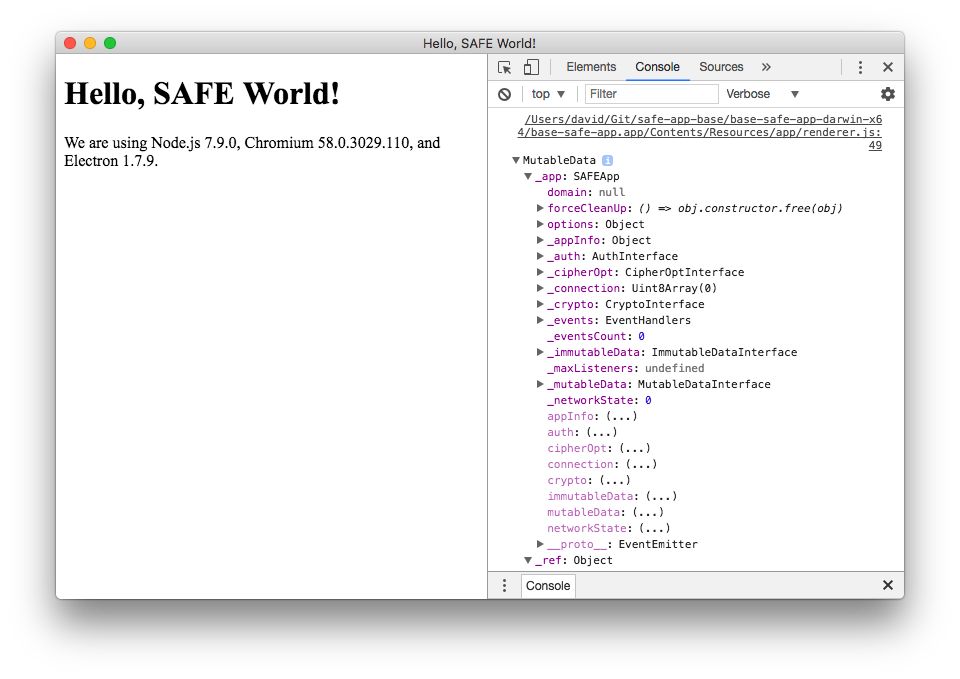
\includegraphics[width=\textwidth]{images/safe-app-base}
		\caption{SAFE App Base with newly created Mutable Data structure}
		\label{fig:safe-app-base}
	\end{center}
\end{figure}

It was a big setback for this project because if this simple example application didn't work then it would prove difficult to implement SAFE Wiki successfully. To help solve this a forum post\cite{safe-app-base-forummacfix} was created to discuss the issue with the community. The best approach would be to fix the example application before attempting the implementation in SAFE Wiki. After some conversation with numerous people I managed to deduce how to solve the problem, I made the fix myself myself\cite{safe-app-base-fix} and it got merged into the ``safe app base'' example application. The working ``safe app base'' can be seen in Figure \ref{fig:safe-app-base}. Problems with URI Schemes cropped up later on in development too, resulting in another forum post\cite{uri-scheme-ubuntu}. This time the issue was with support on Ubuntu. Thanks to the help of the creator of ``safe app base'' the issue was solved quickly.

\section{NFS Emulation}

To support the storage of ZIM files on the SAFE Network, SAFE Wiki makes use of the NFS emulation support that the \textit{Node.js API} has. This ``emulation'' is just a wrapper around Immutable and Mutable Data structures that makes working with ``files'' much easier. In SAFE Wiki nomenclature there is the concept of a \textit{ZIM folder}. This ``folder'' is really a Mutable Data structure that is emulated as a folder through NFS. Within this folder are placed the ZIM files that a given user uploads.

\subsection{ZIM Folder}

Every account on the SAFE Network has a number of Mutable Data structures by default that are called \textit{containers}. These \textit{containers} are similar to a ``home folder'' on a traditional OS in that they give applications structure (guidance) on where to store things. Such containers include: \_public, \_downloads, \_music, \_pictures, \_videos, etc. The ZIM folder that SAFE Wiki uses is stored within the \_public container because data stored within there can be ``un-encrypted'' or '`public'' data. Within the \_public container is placed a key value pairing where the key is ``zim'' and the value is the XOR Address of a Mutable Data structure that is the ZIM folder. When a user creates a ZIM folder they must specify a name. That name is then hashed to give a unique 256-Bit XOR address which is where the Zim folder is then stored. Thus through the name of the ZIM folder another user can locate the ZIM files uploaded by any other user.

\subsection{ZIM Files}

Once a user has created a ZIM folder they are then able to upload ZIM files to the network. This is achieved through the use of the NFS emulation support of the \textit{Node.js API}.  When a user uploads their ZIM file they give it a name, this name is important. This name is the ``file name'' of the file, meaning that within a given ZIM folder the ZIM file is stored against the name the user specifies.

\begin{figure}[h]
	\begin{center}
		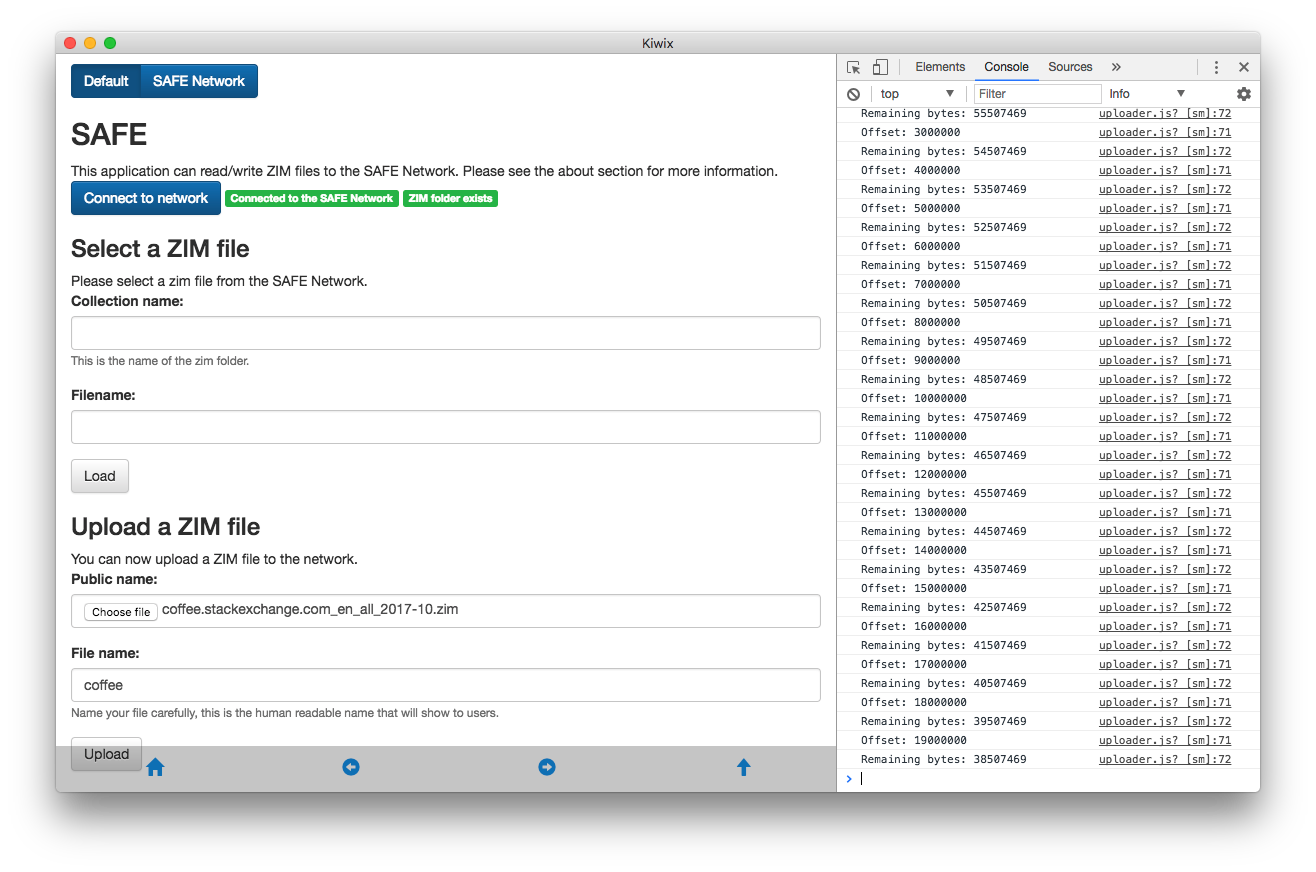
\includegraphics[width=\textwidth]{images/safe-wiki-uploading-coffee}
		\caption{Uploading the Coffee StackOverflow ZIM file to the SAFE Network}
		\label{fig:safe-upload-coffee}
	\end{center}
\end{figure}

To access a ZIM file, all a user has to provide SAFE Wiki with is the name of the ZIM folder and the name of the ZIM file within that folder. This approach means it is easy to share access to ZIM files, as names can be human readable they are as easy to share as website URLs. The resolution of the 256-Bit XOR address of the ZIM Folder is through hashing. As the ZIM folder was stored at the address corresponding to the name specified by the ``owner'', the address is then derivable by anyone else that knows that name. The way this is envisioned to be used is the name of the ZIM folder can correspond to the originator of the content then the filenames follow on logically from that. For example, ``Wikimedia'' could be the name of the ZIM folder then ``Wikipedia'' could be the name of the ZIM file. Meaning a user has two words to type in to browse the latest version of Wikipedia. As things are organised like this it then becomes logical to derive the location of other ZIM files. A user can deduce that to get to ``WikiVoyage'' is as simple as ``Wikimedia'' and ``WikiVoyage'`.

\section{Reading ZIM Files}
 
An important feature that is facilitated through the use of \textit{Data Maps}(Section \ref{subsec:self-encryption-data-map}) is being able to randomly seek through files. The \textit{Data Map} contains enough information about a file that arbitrary bytes can be read without having to download all data chunks. For ZIM files this is important, it is illogical for SAFE Wiki to have to download the entire Wikipedia so a user can browse a single article.

\begin{figure}[h]
	\begin{center}
		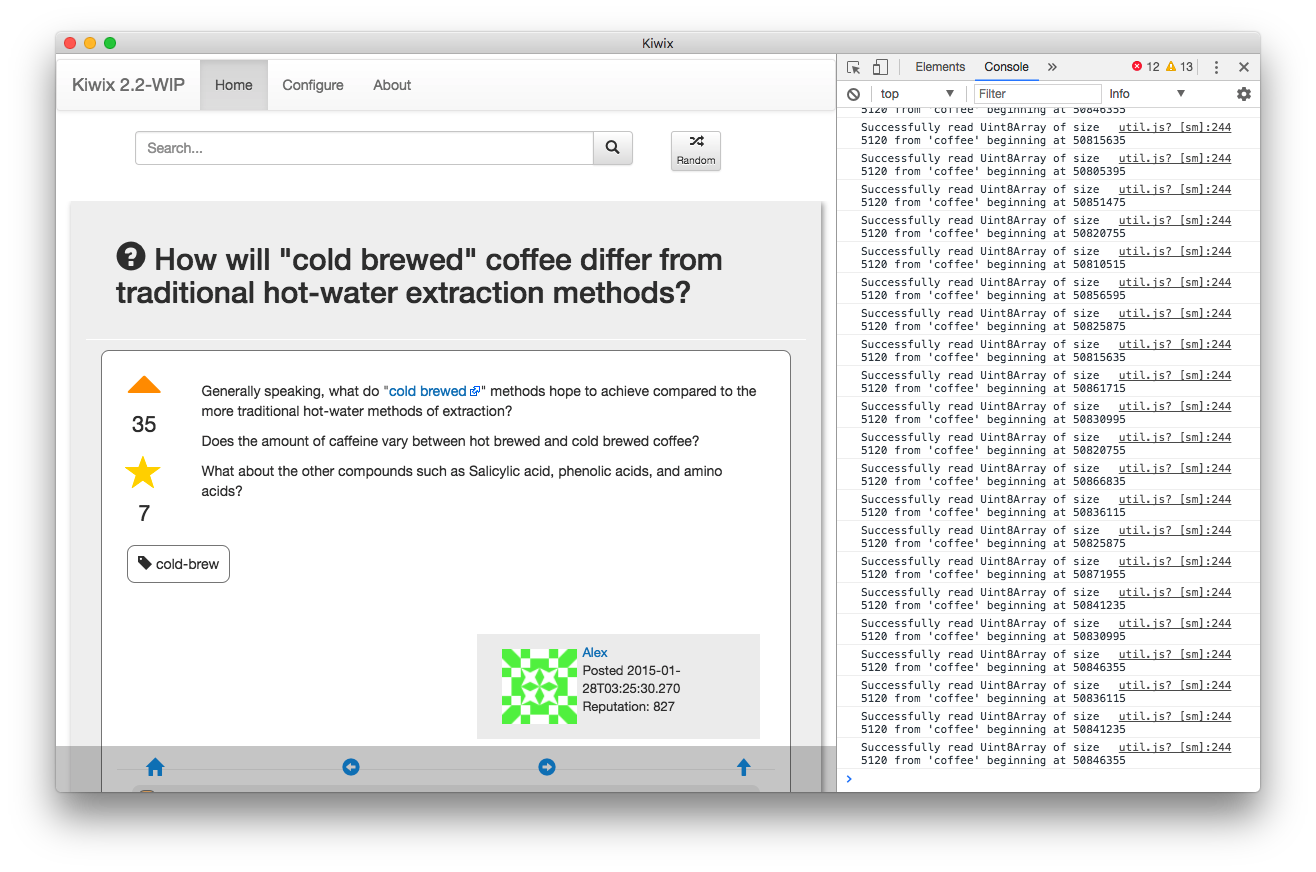
\includegraphics[scale=0.6]{images/safe-wiki-browsing-coffee}
		\caption{Browsing a page from the StackOverflow Coffee ZIM file on the SAFE Network}
		\label{fig:browsing-coffee}
	\end{center}
\end{figure}

Kiwix JS by itself is setup to read ZIM files from local storage. To facilitate reading ZIM files from the SAFE Network, instead of reading a number of bytes (specified by ``begin'' and ``size'' in Figure\ref{fig:zim-read-code}) from local storage, the request is directed to the SAFE Network. Doing it this way is convenient because it doesn't require a complete overhaul of file reading within Kiwix JS. This approach, being more modular in design, means that the original functionality of Kiwix JS is maintained. You can select whether to read files locally or to read them from the SAFE network. The code to perform reading is shown in Figure \ref{fig:zim-read-code}. The \textit{zimFolder} that is a Mutable Data structure is emulated using NFS and the \textit{file} is fetched through the \textit{filename} specified by the user. To then read the required bytes is simple. In Figure \ref{fig:browsing-coffee} the console shows the reads from the network. The API and libraries handle all of the complexities of \textit{Data Maps} for you so reading from the network in this fashion is not complex once all the pieces are in place.

\begin{figure}[h]
\begin{lstlisting}[frame=single]
readZim (zimFolder, filename, begin, size) {
  return new Promise(async (resolve, reject) => {
    try {
      const nfs = zimFolder.emulateAs('NFS')
      let file = await nfs.fetch(filename)
      file = await nfs.open(file, CONSTANTS.FILE_OPEN_MODE.OPEN_MODE_READ)
      let data = await file.read(begin, size)
      file.close()
      resolve(data)
    } catch (error) {
      reject(error)
    }
  })
}
\end{lstlisting}
\caption{Code to read a ZIM file from the SAFE Network}
\label{fig:zim-read-code}
\end{figure}











\chapter{Evaluation}

\chapter{Conclusion}

\section{The Uncertainties of the SAFE Network}

Evaluating the SAFE Network on how it is now does the project an injustice. It is not finished yet and they don't claim it to be. Uncertainties in implementation details, especially \textit{Safecoin}, brings into question how successful the project will be in the long run. Proper incentives for \textit{vault} owners is crucial in the success of the network. The next big step for the project is the implementation of Datachain's (Section \ref{sec:datachain}) and it will be very interesting to see how successful that is. Maidsafe have performed simulations on how \textit{section splits} and \textit{merges} will happen but to see how things handle with a real network will be interesting. There is the real concern of what happens when large parts of the network fail, something that Datachain's hope to address. How effective these mitigation and safety features will be is still to be addressed. Personally I will be very interested to see future work and papers that directly address these issues because they are very complex issues that need to be solved.

The effectiveness of ``Building Applications on the SAFE Network'' is something that can be directly addressed. The infancy of the SAFE Network has made this project difficult. No central source of reliable resources for developers is nightmarish when time is precious such as in building SAFE Wiki. Upon conclusion of this project however SAFE Wiki is a fully functional application that can be used with the current version of the SAFE Network. Assuming that the API won't have any ``breaking'' changes, if and when the SAFE Network fully launches SAFE Wiki will be available for use. People all over the world will be able to access resources like Wikipedia that are hosted on a decentralised and censorship resistant platform.

The SAFE Network ultimately provides an interesting new way to develop applications and services. Developers will have to re-think how they build applications and give proper attention as to how to exploit the characteristics of the SAFE Network to their benefit. Although SAFE Wiki demonstrates that the secure storage and retrieval of data is already possible, more studies and analysis on the feasibility of different applications on the  SAFE Network is needed. Specifically the feasibility of running large websites and services that require extremely fast processing of data needs to be researched fully. The performance of how a world wide SAFE Network with dynamic growth and decay will only be known once it fully launches. It is only then that a true mandate for the use of the SAFE Network can be established. The passion exerted by the team at Maidsafe can only inspire confidence in that they will try their very hardest to achieve all of their goals.

\section{Attribution}

This project would not have been possible without the support of my supervisor Inah Omoronyia. I will be forever grateful for being introduced to the SAFE Network and having my horizons on how applications can built expanded.

I owe gratitude to Maidsafe themselves in that they gave us the opportunity to meet with them at their headquarters in Ayr. The hour we spent together was very illuminating and I truly hope it is not the last interaction that I have with them.

To the forum and community members that answered my queries and questions I owe a great deal of thanks. Most of them are just fellow humans, volunteers who's unwavering passion for the work that Maidsafe is doing really shines through. Without their help and answering of my questions I wouldn't have been able to build SAFE Wiki.

The creators of Kiwix are truly inspiring people. The work that they do in delivering free educational content to the people who most need it is truly inspiring. I hope to be able to contribute something back to their projects in the future. 

\printbibliography

\end{document}
